\documentclass[14pt]{article}
\usepackage{listings}
\usepackage{color}
\usepackage{graphicx}
\usepackage{setspace}

\definecolor{dkgreen}{rgb}{0,0.6,0}
\definecolor{gray}{rgb}{0.5,0.5,0.5}
\definecolor{mauve}{rgb}{0.58,0,0.82}

\lstset{frame=tb,
  language=python,
  aboveskip=3mm,
  belowskip=3mm,
  showstringspaces=false,
  columns=flexible,
  basicstyle={\small\ttfamily},
  numbers=none,
  numberstyle=\tiny\color{gray},
  keywordstyle=\color{blue},
  commentstyle=\color{dkgreen},
  stringstyle=\color{mauve},
  breaklines=true,
  breakatwhitespace=true
  tabsize=3
}







\begin{document}
\title{% 
  \huge Artificial Inteligence \\
  \vspace{20mm}
  \large Course Homework \\
    Problem number 4}

\date{\today}
\maketitle
\begin{center}
\vspace{30 mm}

\title{\huge Student: Marcu Andrei Cristian}
\\\vspace{10 mm}
\title{\huge Computers and Information Technology}
\\\vspace{10 mm}
\title{\huge CEN 2.2 A}
\\\vspace{10 mm}
\title{\huge 2nd Year}
\date{}
\maketitle

\newpage
\section*{Problem statement}
\vspace{20 mm}
C++ function that returns my problem number\\
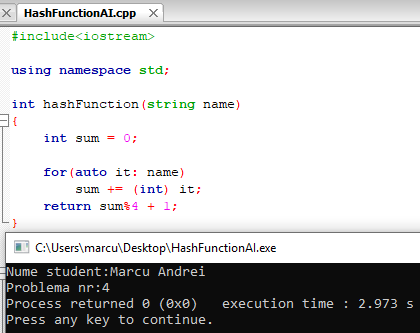
\includegraphics[height=2.7in, width = 4.5in]{problemanr41.png}\\
Python code that computes my problem number\\
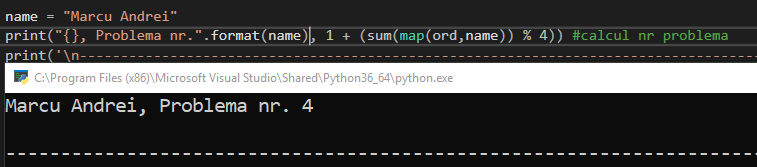
\includegraphics[height=1.5in, width = 6in]{problemanr42.png}\\
\vspace{20 mm}
4.n vehicles occupy squares (1, 1) through (n, 1) (i.e., the bottom row) of
an n×n n grid. The vehicles must be moved to the top row but in reverse
order; so the vehicle i that starts in (i, 1) must end up in (n−i+ 1, n). On each time step, every one of the n vehicles can move one square up, down,
left, or right, or stay put; but if a vehicle stays put, one other adjacent
vehicle (but not more than one) can hop over it. Two vehicles cannot
occupy the same square.
\vspace{5mm}
\\a. Write a detailed formulation for this search problem.
\\b. Identify a suitable search algorithm for this task and explain your
choice.
\\\vspace{10 mm}
a.As we mentioned before we have a matrix which has the first line full of cars, and the goal is to move all the cars in reverse order than the starting one to the last line. We have multiple moves, some of them can move the car one square(LEFT, RIGHT, UP, DOWN) and some of them can move the car two squares(JUMP LEFT, JUMP RIGHT, JUMP UP, JUMP DOWN). There is also a STAY option, which makes the car keep it's current state. So we have 9 possible actions for each car.
\\\vspace{5 mm}
For example for a matrix like this:
\\
1 2 3 4
\\
0 0 0 0
\\
0 0 0 0
\\
0 0 0 0
\\
The answer should be:
\\
0 0 0 0
\\
0 0 0 0
\\
0 0 0 0
\\
4 3 2 1
\\
For this one:
\\
2 1 3
\\
0 0 0
\\
0 0 0
\\
The answer should be:
\\
0 0 0
\\
0 0 0
\\
3 1 2
\\
I'll explain more examples step by step later on my presentation.
\\
Now that we've clarified the Problem Statement we can move on to the implementation, the search algorithm I've used.
\\\vspace{10}
b.I've used the A* search algorithm in order to solve the problem, with multiple heuristics. Some of the heuristics are : Diagonal Distance Manhattan, Distance, Misplaced Cars, Distance between goal and current position, Number of misplaced cars on row and column . All of them will be presented and explained later.
\\\vspace{10 mm}
I've used the framework from our laboratory, which has A* already implemented, so I've adapted this one for our problem. The search algorithm can be found in search.py and the solution for the problem in Cars.py
\newpage
\end{center}

\newpage
\section*{Pseudocode}
First, we need to generate a random initial state. After we've created the initial state we can compute the goal. The function "generate state" handles both of the tasks presented before.

\begin{verbatim}
function generate_state(initial, goal, matrix_size) creates two lists
persistent:initial is initially empty
           goal is initially empty
           matrix size is read from the keyboard
           
for iterator (1, matrix_size ^ 2) step 1 do
  if iterator < matrix_size then
      value <- random value from 1 to matrix_size
      while value in already in initial: 
          value <- random value from 1 to matrix_size
      in initial we add value
  else:
      in initial we add 0
   
for iterator (1, matrix_size ^ 2) step 1 do
   if iterator < pow(matrix_size, 2) - matrix_size then 
      in goal we add 0
   else:
       matrix_size is decremented
       in goal we add initial[matrix_size] 
\end{verbatim}
\\Now that we have a function that generates an initial state and a goal we can move one with the algorithm. The next function is the function that provides all the moves a car can do.
\begin{verbatim}
function actions(state) returns all the possible actions for a car
persistent: possible_actions is a list initialized with ['UP', 'DOWN', 'LEFT', 
'RIGHT', 'JUMPLEFT', 'JUMPRIGHT', 'JUMPUP', 'JUMPDOWN', 'STAY']
            cars is a queue initialized with [1,2,...,matrix_size]
            matrix size is read from the keyboard

x gets the next element from the queue cars
we add x to the queue cars
index <- index of the element x in state
if goal[index] == state[index] then
    possible_actions = ['STAY']
    return possible_actions
if index % matrix_size == 0 or state[index - 1] != 0 then
    from possible_actions we remove 'LEFT'
if index % matrix_size == matrix_size - 1 or state[index + 1] != 0 then
    from possible_actions we remove 'RIGHT'
if index < matrix_size or state[index - matrix_size] != 0 then
    from possible_actions we remove 'UP'
if index > matrix_size^2 - matrix_size - 1) or state[index + matrix_size] != 0 then 
    from possible_actions we remove 'DOWN'
    
if index - 2 >= 0 and index - 1 >= 0 then
    if index % matrix_size == 1 
    or index % matrix_size == 0  
    or state[index-1] == 0 
    or state[index-2] != 0 then
        from possible_actions we remove 'JUMPLEFT'
else:
    from possible_actions we remove 'JUMPLEFT'

if index + 2 < matrix_size * 2 and index+1 < matrix_size * 2 then
    if index % matrix_size == 1 
    or index % matrix_size == 2 
    or state[index+1] == 0 
    or state[index+2] != 0 then
        from possible_actions we remove 'JUMPRIGHT'
else:
    from possible_actions we remove 'JUMPRIGHT'

if index - matrix_size >= 0 and index - 2 * .matrix_size >= 0 then
    if index < 2 * matrix_size 
    or state[index-matrix_size] == 0 
    or state[index - 2 * matrix_size] != 0 then
        from possible_actions we remove 'JUMPUP'
else:
    from possible_actions we remove 'JUMPUP'


if index+matrix_size < matrix_size * 2 
and index+2 * matrix_size < matrix_size * 2 then
    if index > matrix_size^2 - 2 * matrix_size - 1 
    or state[index+matrix_size] == 0 
    or state[index+2 * matrix_size] != 0 then
        from possible_actions we remove 'JUMPDOWN'
else:
    from possible_actions we remove 'JUMPDOWN'
    
return possible_actions

\end{verbatim}
\newpage
\\ Good, now we have a function that returns all the possible actions. Now we should see where those actions will move our car. The next function solves this problem.
\begin{verbatim}
function result(state, action) returns the next state
persistent:new_state is an empty list with the same size as state
           aux is an auxiliary variable we use to interchange two numbers
           neighbour is the new position of the car
           delta is a map which has the same values all time :
{'UP': -matrix_size, 'DOWN': matrix_size, 'LEFT':-1,
'RIGHT':1, 'JUMPLEFT':-2, 'JUMPRIGHT':2, 'JUMPDOWN':2 *
matrix_size, 'JUMPUP':-2 * matrix_size, 'STAY':0}
           matrix_size is the same one we used before
           index is the same one we used before
           action is one of the possible actions declared before
       
neighbour <- index + delta[action] 
aux <- new_state[index]
new_state[index] <- new_state[neighbour]
new_state[neighbour] <- new[state[index]]

return new_state
\end{verbatim}
\\ Now we have all we need for our search algorithm to work. The next functions are used to improve the time in which the search algorithm will solve the problem. The first function is an implementation of Diagonal Distance improved for our problem
\begin{verbatim}
function h(goal, state): returns the value of the heuristic,
the value should be as close as possible to 0

persistent: dx and dy are initially 0
            matrix_size is the same one we used before
            
for i (1, matrix_size + 1) step 1 do
    s <- index of the element i in state
    g <- index of the element i in goal
    dx <- dx + abs((s/matrix_size) - (g/matrix_size)) 
    dy <- dy + abs((s%matrix_size) - (g%matrix_size)) 
return 1 * (dx + dy) + (2 * matrix_size - 2 * 1) * min(dx,dy)
\end{verbatim}
\newpage
\\Another heuristic I've used is the Manhattan distance even though this one isn't as good as Diagonal Distance
\begin{verbatim}
function h(goal, state): return the value of the heuristic,
the value should be as close as possible to 0

for i (1, matrix_size) step 1 do
    s <- index of the element i in state
    g <- index of the element i in goal
    dx <- dx + abs (( s / matrix_size ) - (g / matrix_size))
    dy <- dy + abs (( s % matrix_size ) - (g % matrix_size))
return dx+dy
            
\end{verbatim}
\\I've used 3 more heuristics but the best ones are the one I wrote before. The rest of them are used only to be sure my solution covers many input examples in optimal time.


\newpage
\section*{Application outline}
\vspace{10 mm}
\textcolor{red}{Input} : the program takes as input two tuples that simulate two matrices. This input is generated randomly by the generate\_state function.\\
Example of input for matrix size = 3:\\
initial = [2,1,3,0,0,0,0,0,0]\\
goal = [0,0,0,0,0,0,3,1,2]\\\\
\textcolor{red}{Output} : the output is also a tuple, but it's made to look like a matrix. It shows the matrix after every move of a car.The output is made in the class \textcolor{blue}{Node} from the file \textbf{\textit{search.py}} in the function \textbf{repr(self)}. I also print the tuples but those one are hard to follow. \\
For the input initial = [2,1,3,0,0,0,0,0,0]\\
The last matrix printed will look like:\\
0 0 0\\
0 0 0\\
3 1 2\\
I'll present some step by step outputs in the Experiments and results section.
\\\\
The application is made out of 4 python files, \textbf{\textit{Cars.py}}, \textbf{\textit{main.py}}, \textbf{\textit{search.py}} and \textbf{\textit{utils.py}}.
\\\\
The file \textcolor{red}{Cars.py} contains the solution for the problem and it's made out of the following classes and functions:
\\
\\---class \textcolor{blue}{Cars}, which contains the brain of the problem, the others just extend the class Cars with another heuristic.
\\
This class contains the following functions:
\\ 
\\
-def \textbf{init(self, initial, goal = None)}, the constructor. He is initializing the initial state and the goal, computes the dimension of the matrix, initialises the queue which keeps the cars movements in order with values from 1 to dimension of the matrix, initialises the cost for each movement ( i.e. Left - 1, Right + 1)
\\
\\
-def \textbf{actions(self, state)}, the function that returns all the possible actions a car can make. It checks every situation that can block a car or prevent it from jumping/moving(i.e. getting out of matrix or moving into another car). This function also controls the queue of cars in order to move them in ascending order.
\\
\\
-def \textbf{result(self, state, action)}, returns the new state of the matrix. It takes each of the possible actions returned by the function I've presented above and computes the new state interchanging the car with the empty spot.
\\
\\
-def \textbf{h(self, node)}, the initial heuristic, Misplaced Cars heuristic.
\\
\\--- class \textcolor{blue}{CarsDiagonalDistance}, which extends the class Cars with another function h:
\\
\\
-def \textbf{h(self, node)}, the Diagonal Distance heuristic, modified for our problem.
\\
\\--- class  \textcolor{blue}{CarsMht}, which extends the class Cars with another heuristic h:
\\
\\
-def \textbf{h(self, node)}, the Manhattan Distance heuristic, doesn't work on all the cases because of the jump posibilities.
\\
\\--- class \textcolor{blue}{CarsDist}, which extends the class Cars with another heuristic h:
\\
\\
-def \textbf{h(self, node)}, A heuristic that calculates the sum of the distances from the goal to the current state
\\
\\--- class \textcolor{blue}{CarsMisColRow}, which extends the class Cars with another heuristic h:
\\
\\
-def \textbf{h(self, node)}, A heuristic that computes the number of misplaced cars on each row and column and returns their sum.
\\
\\
And a standalone function that generates a random initial state and the goal for that state
\\
-def \textbf{generatestate(initial, goal, matrix size)}
\\\\
The file \textcolor{red}{search.py} contains the implementation of A* search, recursive best first search, the uninformed best first graph search astar needs,  the pure abstract class that we use to implement our problem, this class is called \textcolor{blue}{Problem} and the class \textcolor{blue}{Node} which was already provided by the framework. I've adapted the way this classes work in order to solve my problem.
\\\\I've modified in the class \textcolor{blue}{Node} the function \textbf{repr(self)} in order to print the matrix which is easily followed instead of the list of actions.
\\\\
The file \textcolor{red}{main.py} has all the function calls and class instances. The main file is also treating the heuristics using exceptions. I've made my code throw an exception when we reach matrix size * matrix size * 1000 iterations because some of the heuristics could take hours to solve an example and other ones can solve it in seconds. Matrix size is also initialized from the keyboard in this file.
\\\\
The file \textcolor{red}{utils.py} is the one provided in the framework and it contains some prerequisites for search.py, some functions that can simplify our job. I didn't change anything in this file

\newpage
\section*{Source Code}
\begin{lstlisting}
#-----------------------------Cars.py-------------------------------
from search import Problem
import math
from queue import *
import random

class Cars(Problem):

    def __init__(self, initial, goal = None):
        """ Define goal state and initialize a problem """
        self.goal = goal
        self.matrix_size = int(math.sqrt(len(initial)))
        self.total_iterations = 0
        self.cars = Queue(self.matrix_size) # o coada in care salvam ordinea in care se muta masinile
        self.delta = {'UP': -self.matrix_size, 'DOWN': self.matrix_size, 'LEFT':-1, 'RIGHT':1, 'JUMPLEFT':-2, 'JUMPRIGHT':2, 'JUMPDOWN':2 * self.matrix_size, 'JUMPUP':-2 * self.matrix_size, 'STAY':0}
        for i in range (1, self.matrix_size+1):
            self.cars.put(i) # umplem coada cu masini de la 1 la matrix_size+1
        Problem.__init__(self, initial, goal)


    def actions(self, state):
        
        possible_actions = ['UP', 'DOWN', 'LEFT', 'RIGHT', 'JUMPLEFT', 'JUMPRIGHT', 'JUMPUP', 'JUMPDOWN', 'STAY']

        x = self.cars.get() #de fiecare data cand scoatem o masina o punem din nou la sfarsit in coada
        self.cars.put(x)
        #aceasta coada ne ajuta sa mentinem ordinea in care se vor efectua miscarile


        self.index = state.index(x)

        if(self.goal[self.index] == state[self.index]): #daca am ajuns la destinatie facem doar STAY
            possible_actions = ['STAY']
            return possible_actions

        if self.index % self.matrix_size == 0 or state[self.index - 1] != 0: #daca suntem pe prima coloana sau daca avem o alta masina in stanga stergem LEFT
            possible_actions.remove('LEFT')

        if self.index % self.matrix_size == self.matrix_size - 1 or state[self.index + 1] != 0: # daca suntem pe ultima coloana sau daca avem masina in dreapta stergem RIGHT
            possible_actions.remove('RIGHT')

        if self.index < self.matrix_size or state[self.index - self.matrix_size] != 0: # suntem pe prima linie sau daca avem masina deasupra stergem UP 
            possible_actions.remove('UP')
            
        if self.index > (pow(self.matrix_size, 2) - self.matrix_size - 1) or state[self.index + self.matrix_size] != 0: # daca suntem pe ultima linie sau daca avem masina sub eliminam DOWN
            possible_actions.remove('DOWN')
        

        if self.index - 2 >= 0 and self.index - 1 >= 0: # verificam daca prin salt masina va iesi din matrice
            #daca suntem pe prima sau a 2-a coloana, daca nu avem masina in stanga sau daca avem masina 2 pozitii in stanga eliminam JUMPLEFT
            if self.index % self.matrix_size == 1 or self.index % self.matrix_size == 0  or state[self.index-1] == 0 or state[self.index-2] != 0:
                possible_actions.remove('JUMPLEFT')
        else:
            possible_actions.remove('JUMPLEFT')
        
        if self.index + 2 < self.matrix_size * 2 and self.index+1 < self.matrix_size * 2: # verificam daca prin salt masina va iesi din matrice
            #daca suntem pe ultima sau penultima coloana, daca nu avem masina in dreapta sau daca avem masina 2 pozitii in dreapta eliminam JUMPRIGHT
            if self.index % self.matrix_size == 1 or self.index % self.matrix_size == 2 or state[self.index+1] == 0 or state[self.index+2] != 0:
                possible_actions.remove('JUMPRIGHT')
        else:
            possible_actions.remove('JUMPRIGHT')
        
        if self.index - self.matrix_size >= 0 and self.index - 2 * self.matrix_size >= 0: # verificam daca prin salt masina va iesi din matrice
            #daca suntem pe prima sau a 2-a linie, daca nu avem masina deasupra sau daca avem masina 2 pozitii mai sus eliminam JUMPUP
            if self.index < 2 * self.matrix_size or state[self.index-self.matrix_size] == 0 or  state[self.index - 2 * self.matrix_size] != 0:
                possible_actions.remove('JUMPUP')
        else:
            possible_actions.remove('JUMPUP')

        if self.index+self.matrix_size < self.matrix_size * 2 and self.index+2 * self.matrix_size < self.matrix_size * 2: # verificam daca prin salt masina va iesi din matrice
            #daca suntem pe ultima sau penultima linie, daca nu avem masina sub sau daca avem masina 2 pozitii mai jos eliminam JUMPDOWN
            if self.index > pow(self.matrix_size, 2) - 2 * self.matrix_size - 1 or state[self.index+self.matrix_size] == 0 or  state[self.index+2 * self.matrix_size] != 0:
                possible_actions.remove('JUMPDOWN')
        else:
            possible_actions.remove('JUMPDOWN')
               
        return possible_actions

    def result(self, state, action):
        """ Given state and action, return a new state that is the result of the action.
        Action is assumed to be a valid action in the state """
        # blank is the index of the blank square
        self.total_iterations += 1 # limita de iteratii
        if(self.total_iterations > pow(self.matrix_size,2) * 1000): # in cazul in care s-a ajuns la nr de iteratii dorit lansam o exceptie pentru a sari peste aceasta executie
            raise Exception

        new_state = list(state) # aici vom salva noul state
       
        neighbour = self.index + self.delta[action] # calculam noua pozitie a masinii si o salvam
        new_state[self.index], new_state[neighbour] = new_state[neighbour], new_state[self.index] # interschimbam pozitia masinei cu noua pozitie

        return tuple(new_state)

    def h(self, node):
        """ Return the heuristic value for a given state. Default heuristic function used is
        h(n) = number of misplaced tiles """

        return sum(s != g for (s, g) in zip(node.state, self.goal)) #euristica initiala, numarul de piese plasate gresit.

class CarsDiagonalDistance(Cars): #euristica optima, este o adaptare a Chebyshev distance pentru operatii de jump.
    def h(self, node):
        dx = 0
        dy = 0
        for i in range(1, self.matrix_size + 1):
            s = node.state.index(i)
            g = self.goal.index(i)
            dx += abs((s//self.matrix_size) - (g//self.matrix_size)) #suma distantelor dintre x-ul curent si destinatie
            dy += abs((s%self.matrix_size) - (g%self.matrix_size)) #suma distantelor dintre y-ul curent si destinatie
        return 1 * (dx + dy) + (2 * self.matrix_size - 2 * 1) * min(dx,dy) # O adaptare a formulei lui Chebyshev pentru distanta, 1 fiind costul pentru o deplasare normala iar 2*matrix_size costul pentru o deplasare de tip JUMP


class CarsMht(Cars): #euristica folosind Manhattan distance, aceasta nu este optima pe toate cazurile deoarece avem si operatii de jump
    def h(self, node):
        return sum( ( abs((s // self.matrix_size) - (g // self.matrix_size)) + abs((s % self.matrix_size) - (g % self.matrix_size)) ) for (s,g) in zip (node.state, self.goal) )



class CarsDist(Cars): #calculeaza distanta dintre piesele asezate gresit si pozitia pe care ar trebui sa o aiba aceste piese. Nu este optima pe majoritatea cazurilor
    def h(self, node):

        dist = 0 # the distance between the misplaced tiles
        for i in node.state:
            if node.state[i] != self.goal[i]: #daca piesa e asezata gresit
                dist += math.fabs(node.state.index(i) - self.goal.index(i)) #calculam distanta dintre aceasta si destinatie

        return dist #returnam suma distantelor
    
        
class CarsMisColRow(Cars):#calculeaza numarul de piese amplasate gresit pe coloana si linie si returneaza suma acestora
    def h(self, node):

        misplaced_row = 0 # number of misplaced tiles on rows
        misplaced_col = 0 # number of misplaced tiles on columns

        for i in range(pow(self.matrix_size, 2)):
            if node.state[i] != self.goal[i]: #daca piesa e asezata gresit
                for j in range(self.matrix_size - 1):

                    if i % self.matrix_size == j: # daca se afla pe coloana j incrementam numarul de piese plasate gresit pe coloana
                        misplaced_col += 1
                    if i // self.matrix_size == j: # daca se afla pe linia j incrementam numarul de piese plasate gresit pe coloana
                        misplaced_row += 1

        total_heurst = misplaced_col + misplaced_row
        
        return total_heurst




def generate_state(initial, goal, matrix_size): # creeaza un input initial random si generaza goal-ul pentru inputul respectiv
    for iterator in range ( pow(matrix_size,2)):
        if iterator < matrix_size: #daca suntem pe prima linie
            value = random.randint(1, matrix_size)
            while value in initial: # daca valoarea generata random exista deja in matrice vom genera pana avem o valoare noua
                value = random.randint(1, matrix_size)
            initial.append(value) # introducem valoarea din lista
        else: #daca nu suntem pe prima linie
            initial.append(0)
        
    for iterator in range (pow(matrix_size,2)):
        if iterator < pow(matrix_size, 2) - matrix_size: #daca nu suntem pe ultima linie
            goal.append(0)
        else: #daca suntem pe ultima linie
            matrix_size -= 1
            goal.append(initial[matrix_size]) #introducem in goal elementul de pe pozitia matrix_size care va fi decrementat la fiecare pas, astfel realizand goal-ul in ordine inversa fata de state-ul initial


\end{lstlisting}
\section*{Experiments and results}
\\\\\\
\begin{center}
Example with Diagonal Distance heuristic
\vspace{10mm}

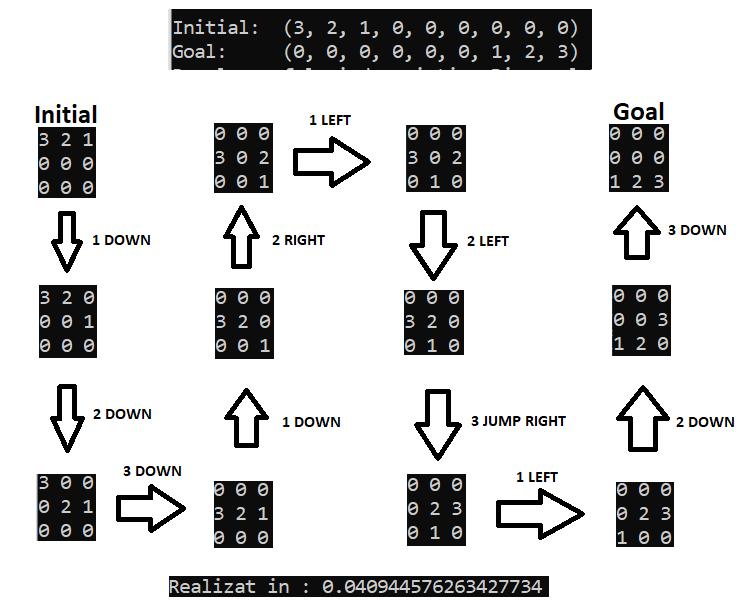
\includegraphics[height=4.5in, width = 5in]{example1.png}\\
\newpage
The same example but with Manhattan Distance heuristic  \\
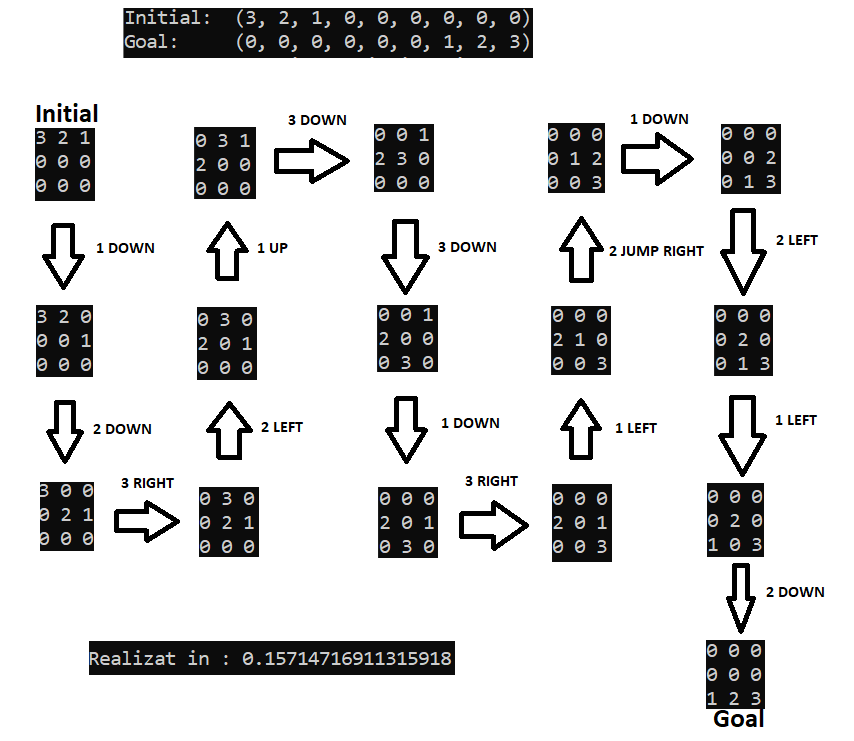
\includegraphics[height=6.1in, width = 6in]{example2.png}\\
The rest of examples will be found in the txt files from the Code directory.
\end{center}\\


\newpage
\section*{Conclusions}
\vspace{20 mm}
Working on this problem, I have acquired lots of knowledge about heuristics and the necessity of those, using multiple heuristics I've realised that a heuristic that overestimates the value can destroy the program and from a 10s execution time it can run for hours. I've also improved my python writing, my main language being C++. I think my code evolved pretty good considering the time I've had to solve the problem. At start it was taking 5 minutes for a 3x3 matrix, now it solves most of these cases in 0,1 seconds. 
\\\vspace{20mm}
\section*{References}
\large https://stackoverflow.com/questions/20547400/why-allowing-diagonal-movement-would-make-the-a-and-manhattan-distance-inadmiss
\\
\\\vspace{6mm}
\\
http://theory.stanford.edu/~amitp/GameProgramming/Heuristics.html
\\
\\\vspace{6mm}
\\
http://www.sharelatex.com

\end{document}